\documentclass[journal]{IEEEtran}

\usepackage{color}
\usepackage{float}
\usepackage{amssymb}
\usepackage{cite}
\usepackage{amsmath}
\usepackage{amsthm}
\newtheorem{Statement}{Statement}
\usepackage{enumerate}
\usepackage{algorithm}
\usepackage{algpseudocode}
\usepackage{graphicx}
\usepackage{epstopdf}
\epstopdfsetup{outdir=./}
\graphicspath{{../Images/}{../}}
\usepackage{booktabs}
\usepackage{multirow}
\usepackage{bm}
\usepackage{url}
\usepackage{tabularx}
\usepackage{placeins}
\usepackage{balance}
\newcommand{\revision}[1]{\textcolor{blue}{#1}}

% Correct bad hyphenation here
\hyphenation{op-tical net-works semi-conduc-tor}

\begin{document}

\title{MAML-Select: An Online Adaptive Client Selection Method for Federated Learning via Meta-Learning}

%\author{Aakash Sharma, Advait Pathak, Ricktho Sarkar, Om Jee Pandey, \textit{Senior Member, IEEE}
%\thanks{A. Sharma, A. Pathak, and R. Sarkar are undergraduate researchers at IIT BHU Varanasi, Varanasi 221005, India.}
%\thanks{O. J. Pandey is with the Department of Electronics Engineering, IIT BHU Varanasi, Varanasi 221005, India (e-mail: omjee.ece@iitbhu.ac.in).}}

\maketitle

% =====================================================================
% ABSTRACT
% =====================================================================
\begin{abstract}
Federated Learning (FL) enables collaborative model training across edge devices\revision{ but} is bottlenecked by statistical and system heterogeneity. \revision{Crucially, the value of each client to the global model evolves as training progresses. Consequently, a fixed selection rule may become stale.} \revision{In this work, we propose \textbf{MAML-Select}, an online adaptive client-selection framework based on Model-Agnostic Meta-Learning (MAML). MAML-Select learns an initialization for a lightweight meta-policy with 4,673 trainable parameters. The policy can be rapidly adapted using recent feedback before ranking candidates for the next FL round.} \revision{Our current evaluation on Fashion-MNIST and CIFAR-10 with 100 heterogeneous clients under non-IID settings ($\alpha = 0.5$) indicates up to a 53\% reduction in cumulative training TFLOPs, a 28.5\% improvement in time-to-accuracy, and a modest accuracy improvement of up to 1.39 percentage points over random FedAvg selection. These gains are practically relevant because they are achieved alongside lower computational demand and faster convergence.} \revision{The TFLOP and simulated-time reductions are proxy indicators of resource efficiency rather than direct measurements of energy consumption or carbon emissions.}
\end{abstract}
\renewcommand\IEEEkeywordsname{Impact Statement}
\begin{IEEEkeywords}
This work addresses the challenge of deploying FL in heterogeneous \revision{environments, such as the} Internet of Vehicles (IoV) and mobile healthcare systems. By introducing the adaptive client selection framework MAML-Select, we \revision{aim to reduce simulated training latency and computational overhead} in distributed learning. The broader impact of this work lies in enabling scalable, adaptive, and \revision{resource-efficient} distributed learning systems, which are critical for next-generation applications, including smart cities, autonomous systems, healthcare monitoring, and industrial \revision{Internet of Things}. \revision{The reported TFLOP and simulated-time reductions are computational-efficiency indicators. They should not be interpreted as direct measurements of electrical energy consumption or carbon emissions. Future work will evaluate hardware-level energy consumption.}


%This enables more scalable and energy-efficient privacy-preserving AI on resource-constrained edge devices.
\end{IEEEkeywords}
\renewcommand\IEEEkeywordsname{Index Terms}
\begin{IEEEkeywords}
Federated learning, client selection, meta-learning, and computational efficiency.
\end{IEEEkeywords}
% =====================================================================
% I. INTRODUCTION
% =====================================================================
\section{Introduction}

\IEEEPARstart{F}{ederated} Learning (FL)~\cite{mcmahan2017communication} has emerged as \revision{an important} framework for privacy-preserving distributed intelligence. \revision{Clients train models locally and share only model updates with a central server. FL clients vary in hardware capabilities, network conditions, and local data distributions. This heterogeneity creates two coupled challenges. Statistical heterogeneity causes client drift under non-IID data}~\cite{karimireddy2020scaffold}. \revision{System heterogeneity allows stragglers to dictate round latency in synchronous protocols. Recent IEEE TAI studies examine server-side learning under non-IID data}~\cite{mai2024study}, \revision{adaptive handling of stragglers}~\cite{tapwal2026stragglers}, \revision{and asynchronous learning with heterogeneous datasets}~\cite{forootani2026asynchronous}. \revision{Recent work also revisits the definition of non-IID data for computer-vision tasks}~\cite{borazjani2026redefining} \revision{and identifies critical learning periods in which client-selection decisions disproportionately affect final model quality}~\cite{yan2023criticalfl}. Despite these advances, the fundamental problem of \textit{whom to select} for each training round remains an open challenge.

Client selection, the process of choosing a subset $\revision{\mathcal{S}_t} \subset \{1, \ldots, N\}$ each round, is thus a focal point of FL research. \revision{A client that is useful early in training may become redundant later. Conversely, a previously overlooked client may become important.} System-aware methods such as FedCS~\cite{nishio2019client} maximize throughput\revision{. However, they may bias the model against} slow yet data-rich clients. Utility-aware methods such as Oort~\cite{lai2021oort} and FedCor~\cite{tang2022fedcor} prioritize statistical information gain\revision{. Some utility-aware methods incur high latency or cubic computational complexity} $\mathcal{O}(N^3)$. Reinforcement Learning approaches~\cite{wang2020optimizing} model the selection process as a Markov decision problem (MDP)\revision{ and adapt through interaction with the environment}. Recent work has further explored contextual bandit approaches~\cite{pan2024contextual} and gradient compression with client selection~\cite{xu2024federated}. More recently, CriticalFL~\cite{yan2023criticalfl} exploits critical learning periods to time client participation, and FedGCS~\cite{ning2024fedgcs} recasts selection as a generative optimization problem. \revision{These approaches address important aspects of client selection. However, an efficient round-by-round mechanism for adapting the ranking policy to evolving client utility remains underexplored.}

\revision{In this paper, we propose MAML-Select, a client-selection framework based on Model-Agnostic Meta-Learning (MAML)}~\cite{finn2017model}. \revision{MAML-Select learns an initialization for a policy network. Recent feedback is used to rapidly adapt the policy before the next client-ranking decision. Unlike RL-based and contextual-bandit selectors, our focus is rapid gradient-based adaptation of the ranking policy across FL rounds. This is also distinct from FL personalization methods}~\cite{fallah2020personalized}. \revision{Those methods adapt model weights for individual clients. MAML-Select applies meta-learning to the client-selection policy itself. This joint objective is relevant when devices have limited compute, round deadlines are strict, or connectivity is intermittent. In these settings, a modest accuracy gain is valuable when accompanied by faster convergence and lower cumulative computation.} The major contributions can be summarized as follows.
\begin{enumerate}
		\item We formulate the FL client selection problem as a meta-learning task and introduce the \textbf{MAML-Select} algorithm with \revision{rapid gradient-based} adaptation for online client selection.
		\item We demonstrate that MAML-Select \revision{\textit{reduces cumulative training TFLOPs} by 53\% and accelerates convergence by 28.5\%, providing a resource-efficient approach for heterogeneous edge computing}.
	\item Extensive experiments on Fashion-MNIST and CIFAR-10 under non-IID settings ($\alpha = 0.5$) confirm that MAML-Select achieves up to 1.39\% accuracy improvement over FedAvg while outperforming baselines (FedCS, Oort, FedCor) in efficiency.
\end{enumerate}

% =====================================================================
% II. RELATED WORK
% =====================================================================
\section{Related Work}
This section categorizes existing client selection literature into three paradigms and situates MAML-Select within the broader landscape.

\subsubsection{System-Aware Selection}
Early FL research addressed the ``straggler effect,'' where random selection leads to significant idle time. FedCS~\cite{nishio2019client} \revision{selects clients under resource constraints so that the server can aggregate as many updates as possible.} \revision{TiFL}~\cite{chai2020tifl} \revision{divides clients into performance tiers and adaptively updates its tiering using observed training performance and accuracy. Recent IEEE TAI work introduces explainability-driven adaptive handling of stragglers in resource-constrained systems}~\cite{tapwal2026stragglers} \revision{and asynchronous learning for heterogeneous datasets}~\cite{forootani2026asynchronous}. \revision{These methods directly address resource heterogeneity. Their primary mechanisms differ from the round-by-round policy adaptation considered here.}

\subsubsection{Data-Aware and Utility-Based Selection}
Oort~\cite{lai2021oort} \revision{improves time-to-accuracy by prioritizing clients with useful data and the capability to train quickly.} FedCor~\cite{tang2022fedcor} \revision{models correlations between client losses with a Gaussian Process and selects clients that are expected to reduce the global loss.} \revision{FedCG}~\cite{xu2024federated} \revision{jointly optimizes adaptive client selection and gradient compression under heterogeneous edge conditions.} CriticalFL~\cite{yan2023criticalfl} \revision{uses critical learning periods to guide participation.} FedGCS~\cite{ning2024fedgcs} \revision{recasts client selection as a generative task and performs gradient-based optimization in a continuous representation space. FedImp uses impurity-based aggregation weights to improve convergence under heterogeneous data}~\cite{tran2026fedimp}. \revision{These methods improve FL through utility modeling, period awareness, combination search, or aggregation weighting. MAML-Select instead targets rapid adaptation of the ranking policy from recent feedback as client utility evolves.}

\subsubsection{Learning-Based and Meta-Learning Approaches}
\revision{FAVOR}~\cite{wang2020optimizing} \revision{uses deep Q-learning to select clients and counterbalance bias from non-IID data.} \revision{Pan et al.}~\cite{pan2024contextual} \revision{formulate client selection as a neural contextual combinatorial bandit and use locality-sensitive hashing to extract client features. Kazemi et al. use deep reinforcement learning for robust peer-to-peer selection under data-poisoning attacks}~\cite{kazemi2026robust}. \revision{Arisdakessian et al. introduce an inclusive client-selection framework that targets participation fairness}~\cite{arisdakessian2026vox}. \revision{On the personalization front, Fallah et al.}~\cite{fallah2020personalized} \revision{use MAML to learn an initial shared model that each client can adapt to its local data. Beyond selection-policy design, SCAFFOLD}~\cite{karimireddy2020scaffold} \revision{uses control variates to address client drift.}

\revision{Table~\ref{tab:related_work_comparison} consolidates these distinctions. For methods without a stated closed-form selection complexity, it reports the dominant server-side operation.}

\begin{table*}[!t]
    \color{blue}
    \caption{Comparison of representative methods and MAML-Select.}
    \label{tab:related_work_comparison}
    \centering
    \scriptsize
    \setlength{\tabcolsep}{3pt}
    \renewcommand{\arraystretch}{1.15}
    \begin{tabularx}{\textwidth}{lXXXX}
        \toprule
        \textbf{Method} & \textbf{Primary objective} & \textbf{Adaptation mechanism} & \textbf{Selection complexity or dominant operation} & \textbf{Optimization strategy} \\
        \midrule
        FedCS~\cite{nishio2019client} & Increase feasible updates under resource constraints & Resource estimates before selection & Resource-constrained subset search & Deadline-aware scheduling \\
        TiFL~\cite{chai2020tifl} & Mitigate stragglers while preserving accuracy & Online tier updates & Tiering and probabilistic sampling & Adaptive tier-based selection \\
        Oort~\cite{lai2021oort} & Improve time-to-accuracy & Utility and speed feedback & Utility scoring and guided sampling & Exploration and exploitation \\
        FedCor~\cite{tang2022fedcor} & Accelerate convergence under non-IID data & Loss-correlation model & Gaussian-Process covariance operations & GP-based active selection \\
        FAVOR~\cite{wang2020optimizing} & Counterbalance non-IID bias & Experience-driven policy updates & DQN inference and training & Deep Q-learning \\
        NCCB~\cite{pan2024contextual} & Learn contextual client combinations & Client features and reward feedback & LSH feature extraction and bandit updates & Neural contextual combinatorial bandit \\
        FedCG~\cite{xu2024federated} & Couple selection and gradient compression & Capability-aware compression updates & Submodular optimization and linear programming & Joint iterative optimization \\
        CriticalFL~\cite{yan2023criticalfl} & Exploit critical learning periods & Period-aware participation & Base-selector dependent & Selector augmentation \\
        FedGCS~\cite{ning2024fedgcs} & Optimize client combinations & Search in a learned continuous space & Latent-space optimization and beam search & Gradient-based generative selection \\
        Kazemi et al.~\cite{kazemi2026robust} & Improve robustness under poisoning attacks & Experience-driven policy updates & Deep-RL inference and training & Deep reinforcement learning \\
        Vox Populi~\cite{arisdakessian2026vox} & Promote fair and inclusive participation & Fairness-aware client selection & Framework-dependent & Inclusive selection framework \\
        \textbf{MAML-Select} & Adapt rankings under evolving client utility & Fast adaptation from recent round feedback & $\mathcal{O}(N|\phi|)$ scoring plus a gradient-adaptation step & Gradient-based meta-learning \\
        \bottomrule
    \end{tabularx}
\end{table*}

\revision{\textbf{Difference between MAML-Select and prior work.} Personalization approaches adapt a model or client-specific parameters. MAML-Select instead meta-learns the selection policy $h_\phi$. Unlike heuristic, RL, contextual-bandit, and generative selectors, it uses a MAML inner update to adapt the ranking policy from recent feedback before the next decision. Its intended contribution is rapid policy adaptation under evolving client utility, rather than personalized model training.}

% =====================================================================
% III. SYSTEM MODEL AND PROBLEM FORMULATION
% =====================================================================
\section{System Model and Problem Formulation}
\revision{We consider a central server and $N$ heterogeneous clients indexed by $\mathcal{N} = \{1, 2, \ldots, N\}$. Client $i$ stores a local dataset $\mathcal{D}_i$ with $n_i$ samples.} The global objective is to minimize the empirical risk over the distributed data as
\begin{equation}
	\min_{\theta \in \mathbb{R}^d} F(\theta) = \sum_{i=1}^{N} \frac{n_i}{n} F_i(\theta),
	\label{eq:global_objective}
\end{equation}
\revision{where $\theta \in \mathbb{R}^d$ denotes the global model, $n = \sum_{i=1}^{N} n_i$, and $F_i(\theta) = \frac{1}{n_i} \sum_{j=1}^{n_i} \ell(\theta; x_{i,j}, y_{i,j})$ is the local empirical risk.}

\revision{At round $t$, let $\mathcal{A}_t \subseteq \mathcal{N}$ denote the available clients and $\mathcal{S}_t \subseteq \mathcal{A}_t$ the selected cohort. Client $i$ has latency $T_{i,t}=T_{i,t}^{comp}+T_{i,t}^{comm}$, where $T_{i,t}^{comp} = \frac{E n_i C_{model}}{f_{i,t}}$ and $T_{i,t}^{comm} = \frac{M}{B_{i,t}} + \delta_{i,t}$. Here, $E$ is the number of local epochs, $C_{model}$ is the number of FLOPs per sample, $f_{i,t}$ is the compute rate, $M$ is the update size, $B_{i,t}$ is the uplink bandwidth, and $\delta_{i,t}$ is the propagation delay. In synchronous FL, the slowest selected client determines the round latency:}
\begin{equation}
	\color{blue}
	T_t^{round} = \max_{i \in \mathcal{S}_t} T_{i,t},
	\label{eq:round_latency}
\end{equation}
\revision{We report simulated latency and TFLOPs as computational proxies. We do not treat them as direct measurements of electrical energy.}

\revision{Let $a_{i,t}$ indicate whether client $i$ is selected. Under policy $\pi_\phi$, the constrained client-selection problem is}
\begin{equation}
	\color{blue}
	\begin{aligned}
		\min_{\pi_\phi}\quad & \sum_{t=1}^{T} \left[F(\theta_{t+1}) + \lambda T_t^{round}\right] \\
		\text{s.t.}\quad & \sum_{i=1}^{N} a_{i,t}=K,\quad a_{i,t}\in\{0,1\}, \\
		& a_{i,t}\leq \mathbf{1}\{i\in\mathcal{A}_t\},\quad
		\mathcal{S}_t=\{i:a_{i,t}=1\}.
	\end{aligned}
	\label{eq:bi_objective}
\end{equation}
\revision{Here, $K$ is the cohort size, $T$ is the number of rounds, and $\lambda \geq 0$ controls the latency--loss trade-off. A larger $\lambda$ places more emphasis on latency, while $\lambda=0$ yields loss-only selection. We assume $|\mathcal{A}_t|\geq K$. The model $\theta_{t+1}$ results from local training and aggregation over $\mathcal{S}_t$. The problem remains challenging because the action space is combinatorial and client utility evolves during training.}

% =====================================================================
% IV. METHODOLOGY: MAML-SELECT
% =====================================================================
\section{Methodology: MAML-Select Algorithm}
\revision{Building on~\eqref{eq:bi_objective}, MAML-Select treats client selection as a meta-learning problem. Client utility changes as training progresses. However, the mechanism for selecting useful clients from recent feedback can be learned.}

\subsubsection{State Space}
\revision{The server constructs a state vector $\bm{s}_{i,t} \in \mathbb{R}^6$ for each client $i$ at round $t$. It contains local training loss $\hat{L}_{i,t}$, gradient norm $\|\nabla F_i\|_2$, estimated latency $\hat{T}_{i,t}$, battery level $b_{i,t}$, selection frequency $q_{i,t}$, and staleness $\tau_{i,t}$ (rounds since last selected)}~\cite{wang2020optimizing, lai2021oort}. \revision{Loss and gradient norm characterize statistical utility. Latency and battery level characterize system constraints. Selection frequency and staleness expose participation imbalance. Each FL round $t$ is treated as a task $\mathcal{T}_t$. The goal is to rank clients so that the top-$K$ cohort minimizes the per-round cost.}

MAML~\cite{finn2017model} is leveraged to train a meta-policy network $h_\phi(\bm{s}_{i,t})$, parameterized by $\phi$, that learns an initialization adaptable to the current round using data from the preceding round. \revision{The policy is a $6$-$64$-$64$-$1$ multilayer perceptron with ReLU activations and 4,673 trainable parameters.} The support set represents the past experience: $\mathcal{D}_{sup}(t) = \{(\bm{s}_{i,t-1}, c_{i,t-1}) \mid i \in \revision{\mathcal{S}_{t-1}}\}$, containing client states and observed costs from round $t-1$. \revision{The candidate set represents the current decision: $\mathcal{D}_{cand}(t) = \{\bm{s}_{i,t} \mid i \in \mathcal{A}_t\}$, containing the states of available clients.}

\subsubsection{Cost Function}
\revision{The per-client cost $c_{i,t}$ supplies feedback to the ranking policy. Consistent with~\eqref{eq:bi_objective}, it is defined as}
\begin{equation}
	\color{blue}
	c_{i,t} = \lambda \underbrace{\max(0, T_{i,t} - T_{target})}_{\text{latency penalty}} - \underbrace{\Delta_{i,t}}_{\text{local loss reduction}}.
	\label{eq:cost}
\end{equation}
\revision{Here, $\Delta_{i,t}=\hat{L}_{i,t}^{before}-\hat{L}_{i,t}^{after}$ is the observed local loss reduction for selected client $i$. It is a client-level proxy for statistical utility and does not require a server-held validation set. The target $T_{target}$ is a soft deadline. Minimizing $c_{i,t}$ favors lower latency and larger local loss reduction.}

\subsection{The MAML-Select Algorithm}
The algorithm proceeds in three phases per round:

\textbf{Phase~1 (Inner Loop Adaptation (Look-Ahead)):}
At the start of round $t$, \revision{the server adapts the meta-policy $\phi_t$ on $\mathcal{D}_{sup}(t)$ using one gradient-descent step:}
\begin{equation}
	\color{blue}
		\phi'_t = \phi_t - \beta \nabla_{\phi_t} \mathcal{L}_{sup}(h_{\phi_t};\mathcal{D}_{sup}(t)),
		\label{eq:inner_loop}
\end{equation}
where $\mathcal{L}_{sup}$ is the MSE loss between predicted scores and observed costs from round $t-1$, and $\beta$ is the inner learning rate.

{\color{blue}
\begin{Statement}
Let $g_t(\phi)=\mathcal{L}_{sup}(h_\phi;\mathcal{D}_{sup}(t))$. If $g_t$ is $L$-smooth and $0<\beta<2/L$, the inner update in~\eqref{eq:inner_loop} satisfies
\[
g_t(\phi'_t) \leq g_t(\phi_t)
-\beta\left(1-\frac{L\beta}{2}\right)
\|\nabla g_t(\phi_t)\|_2^2.
\]
\end{Statement}
This standard descent bound shows why recent feedback can improve the round-specific policy before ranking current candidates. It motivates rapid adaptation. It is not a global FL convergence guarantee.
}

\textbf{Phase~2 (Client Selection):}
\revision{The adapted policy $h_{\phi'_t}$ scores the available clients and selects the $K$ clients with the lowest predicted costs:}
\begin{equation}
	\color{blue}
	\mathcal{S}_t = \operatorname{Top-}K_{i \in \mathcal{A}_t} \left( -h_{\phi'_t}(\bm{s}_{i,t}) \right).
	\label{eq:selection}
\end{equation}

\textbf{Phase~3 (FL Execution and Outer Loop Update):}
\revision{The selected clients perform standard FL training. Their observed costs form $\mathcal{D}_{query}(t)=\{(\bm{s}_{i,t},c_{i,t})\mid i\in\mathcal{S}_t\}$. The query loss is also mean squared error. The meta-policy is updated on this query set:}
\begin{equation}
		\color{blue}
		\phi_{t+1} \leftarrow \phi_t - \eta \nabla_{\phi'_t} \mathcal{L}_{query}(h_{\phi'_t}; \mathcal{D}_{query}(t)),
		\label{eq:outer_loop}
\end{equation}
\revision{where $\eta$ is the meta-learning rate. We use the first-order MAML approximation}~\cite{nichol2018first}. \revision{It applies the query gradient at $\phi'_t$ and omits second-order derivatives. The full procedure is detailed in Algorithm~\ref{alg:maml_select} and illustrated in Fig.~\ref{fig:model_diagram}.}

\begin{figure}[!t]
	%\centering
	%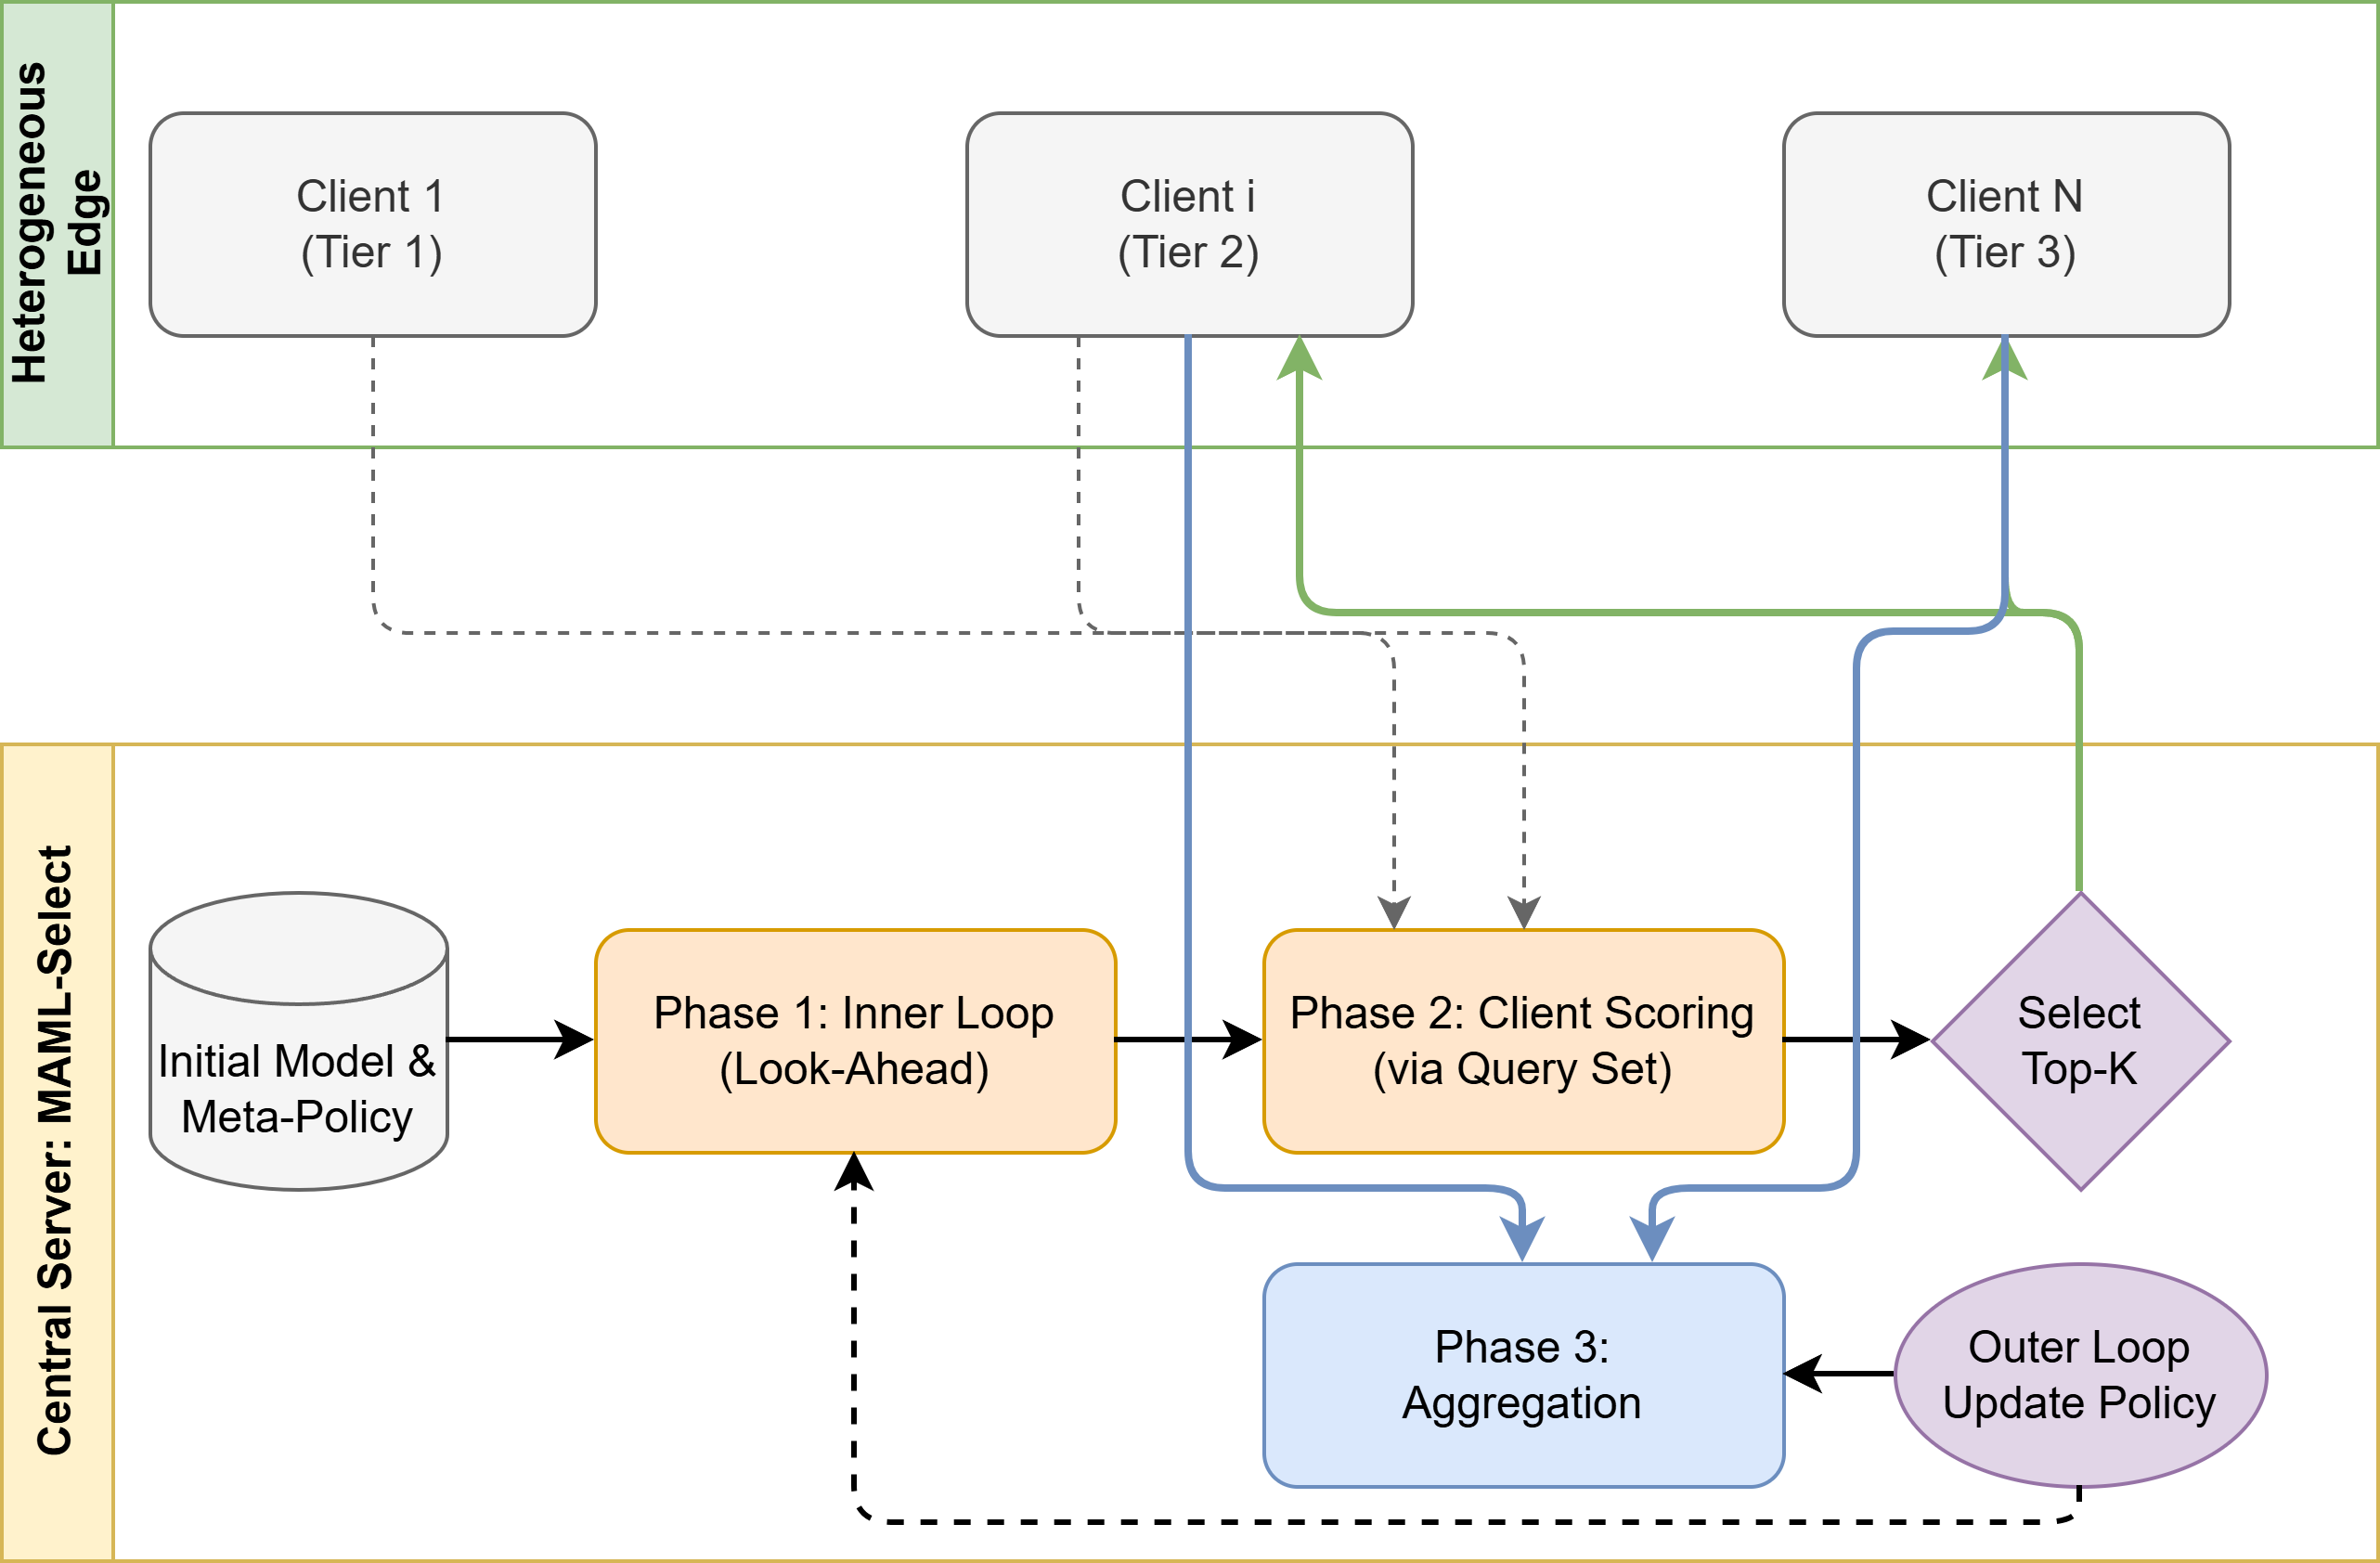
\includegraphics[width=\columnwidth]{Infographic_final.png}
    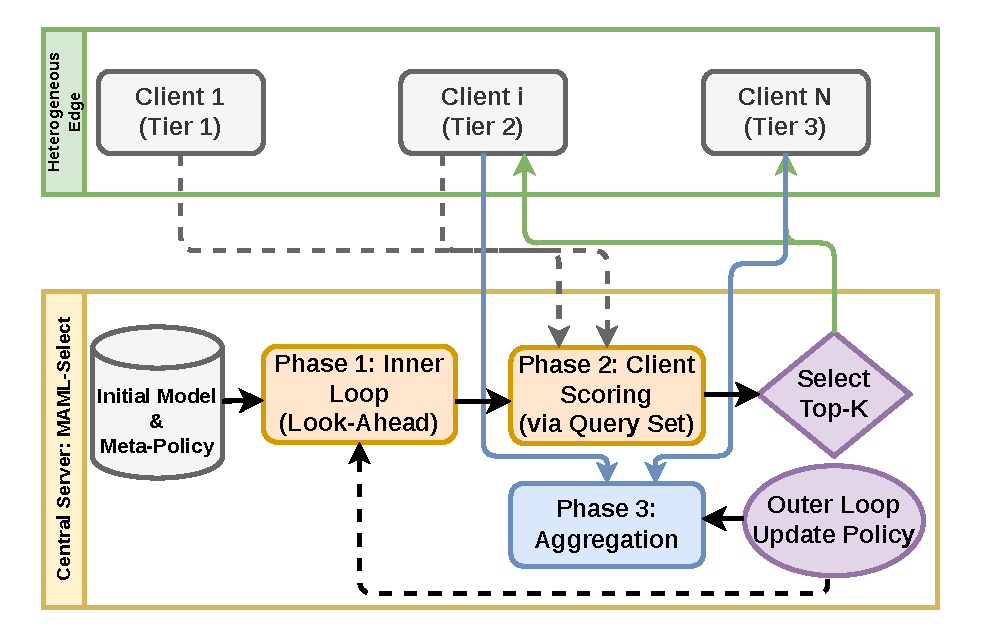
\includegraphics[width=\columnwidth, trim={0.25cm 0.25cm 0.25cm 0.25cm},clip]{MAML.pdf}
		\caption{\small \revision{MAML-Select framework. The server adapts the meta-policy on the previous round's support set, ranks current candidates, and performs a first-order meta-update on observed query-set costs.}}
	\label{fig:model_diagram}
\end{figure}

\begin{algorithm}[!t]
	\caption{MAML-Select Algorithm}
	\label{alg:maml_select}
	\begin{algorithmic}[1]
		\small
		\State \textbf{Initialize:} Global model $\theta_0$; meta-policy parameters $\phi$; inner LR $\beta$; outer LR $\eta$; trade-off $\lambda$.
		\For{round $t = 1, \ldots, T$}
		\State Server broadcasts global model $\theta_t$ to all clients.
		\State Collect state vectors $\bm{s}_{i,t}$ from available clients.
		\If{$t > 1$}
		\State \texttt{// Phase 1: Inner Loop Adaptation}
		\State Construct $\mathcal{D}_{sup}$ from round $t-1$ results.
			\State \revision{Compute fast weights $\phi'_t$ using Eq.~\ref{eq:inner_loop}.}
		\Else
		\State $\phi'_t \leftarrow \phi_t$ \quad \texttt{// No adaptation for the first round}
		\EndIf
		\State \texttt{// Phase 2: Client Selection}
			\State \revision{Score clients: $\text{score}_i = h_{\phi'_t}(\bm{s}_{i,t})$ for all $i \in \mathcal{A}_t$.}
			\State \revision{Select lowest-cost clients: $\mathcal{S}_t \leftarrow \operatorname{Top-}K(-\text{scores})$.}
			\State \texttt{// FL Training Round}
				\State \revision{Receive local updates $\{\Delta\theta_{i,t}\}_{i \in \mathcal{S}_t}$, local losses, and system metrics.}
			\State \revision{Aggregate: $\theta_{t+1} \leftarrow \theta_t + \sum_{i \in \mathcal{S}_t} \frac{n_i}{\sum_{j \in \mathcal{S}_t}n_j}\Delta\theta_{i,t}$.}
			\State \texttt{// Phase 3: Outer Loop Meta-Update}
			\State Compute costs $c_{i,t}$ using Eq.~\ref{eq:cost} for $i \in \revision{\mathcal{S}_t}$.
			\State Construct $\mathcal{D}_{query}(t) = \{(\bm{s}_{i,t}, c_{i,t}) \mid i \in \revision{\mathcal{S}_t}\}$.
				\State \revision{Meta-update: $\phi_{t+1} \leftarrow \phi_t - \eta \nabla_{\phi'_t} \mathcal{L}_{query}(h_{\phi'_t};\mathcal{D}_{query}(t))$.}
		\EndFor
	\end{algorithmic}
\end{algorithm}

\revision{MAML-Select differs from fixed-rule selectors because its ranking policy is adapted before each decision. It also differs from RL selectors because the update is an explicit gradient step on recent support feedback. The method is designed for rapidly changing client utility.}

\subsubsection{Computational Complexity}
\revision{The meta-policy $h_\phi$ is a lightweight MLP with 4,673 parameters. Scoring $N$ available clients costs $\mathcal{O}(N|\phi|)$. One support-set adaptation and one query-set meta-update over a cohort of size $K$ cost $\mathcal{O}(K|\phi|)$. The total server-side policy cost per round is therefore $\mathcal{O}((N+K)|\phi|)$, excluding local model training.}

% =====================================================================
% V. EVALUATION AND RESULTS
% =====================================================================
\section{Evaluation and Results}

We evaluate on two benchmarks: Fashion-MNIST using LightCNN-9~\cite{wu2018light} (lightweight IoT task) and CIFAR-10 using ResNet18~\cite{he2016deep} (complex vision task). $N = 100$ clients are simulated with non-IID data partition (Dirichlet $\alpha = 0.5$)\revision{~\cite{hsu2019measuring}}, selecting $K = 10$ clients per round for $T = 200$ rounds with $E = 5$ local epochs and batch size 32. \revision{Compute rates follow three AI-Benchmark tiers~\cite{ignatov2018ai}: Tier~1 (20\%, $1.0\times$), Tier~2 (50\%, $2.0\times$), and Tier~3 (30\%, $4.0\times$).} The target latency deadline $T_{target}$ is set to the average round latency of Tier~2 clients, and the trade-off parameter $\lambda = 0.5$. Baselines include FedAvg~\cite{mcmahan2017communication} (random selection), FedCS~\cite{nishio2019client} (system-aware deadline-constrained), Oort~\cite{lai2021oort} (utility-based with importance sampling), TiFL~\cite{chai2020tifl} (tier-based), and FedCor~\cite{tang2022fedcor} (correlation-based via Gaussian Processes).

\subsection{\revision{Computational Cost}}
\revision{We estimate the client-training computation required for convergence. The cumulative cost is}
\begin{equation}
		\text{TFLOPs}_{total} = \sum_{t=1}^{T_{conv}} \sum_{i \in \revision{\mathcal{S}_t}} E \cdot n_i \cdot C_{model} \times 10^{-12}.
	\label{eq:tflops}
\end{equation}
For ResNet18 on CIFAR-10, the cost per client per round is approximately \revision{4.13 TFLOPs ($\approx 5.46$ GFLOPs/image $\times$ 500 images $\times$ 5 epochs)}.

\revision{Table~\ref{tab:tflops_analysis} reports the current computation estimates for reaching 88\% accuracy on CIFAR-10. MAML-Select reaches the target in 140 rounds, compared with more than 300 rounds for FedAvg. This corresponds to a 53\% reduction in cumulative TFLOPs. The meta-update overhead ($\varepsilon \approx 0.001$ GFLOPs) is small compared with client-side training. FedCS does not reach the target, whereas Oort yields a 40\% reduction. TFLOPs and simulated time characterize computational efficiency only. They do not establish electrical-energy or carbon savings.}

\begin{table}[!t]
		\caption{\small \revision{Current computational-cost estimate to convergence (target: 88\% accuracy on CIFAR-10).}}
	\centering
	\resizebox{\columnwidth}{!}{
		\begin{tabular}{@{}lcccc@{}}
			\toprule
				\textbf{Method} & \textbf{Rounds} & \textbf{\revision{Cost/Round (TFLOPs)}} & \textbf{\revision{Total TFLOPs}} & \textbf{Saving} \\
			\midrule
			FedAvg & $>300$ & 41.3 & $>12{,}390$ & Baseline \\
			FedCS  & DNR    & 41.3 & N/A & N/A \\
			Oort   & 180    & 41.3 & 7,434 & 40\% \\
			\textbf{MAML-Select} & \textbf{140} & 41.3 + $\varepsilon$ & \textbf{5,782} & \textbf{53\%} \\
			\bottomrule
				\multicolumn{5}{l}{\footnotesize DNR = Did Not Reach target. $\varepsilon$ denotes negligible meta-overhead ($\sim$0.001 GFLOPs).}
		\end{tabular}
	}
	\label{tab:tflops_analysis}
    \vspace{-1em}
\end{table}

\subsection{Efficiency and Time-to-Accuracy}
\revision{Fig.~\ref{fig:efficiency_comparison} depicts accuracy as a function of simulation time and computation. Simulation time denotes accumulated modeled round latency from~\eqref{eq:round_latency}. TFLOPs denote cumulative client-training operations. On Fashion-MNIST, MAML-Select reaches 70\% accuracy approximately 28.5\% faster than FedAvg. On CIFAR-10, the current results show fewer cumulative TFLOPs for MAML-Select.}

\begin{figure}[!t]
		\centering
		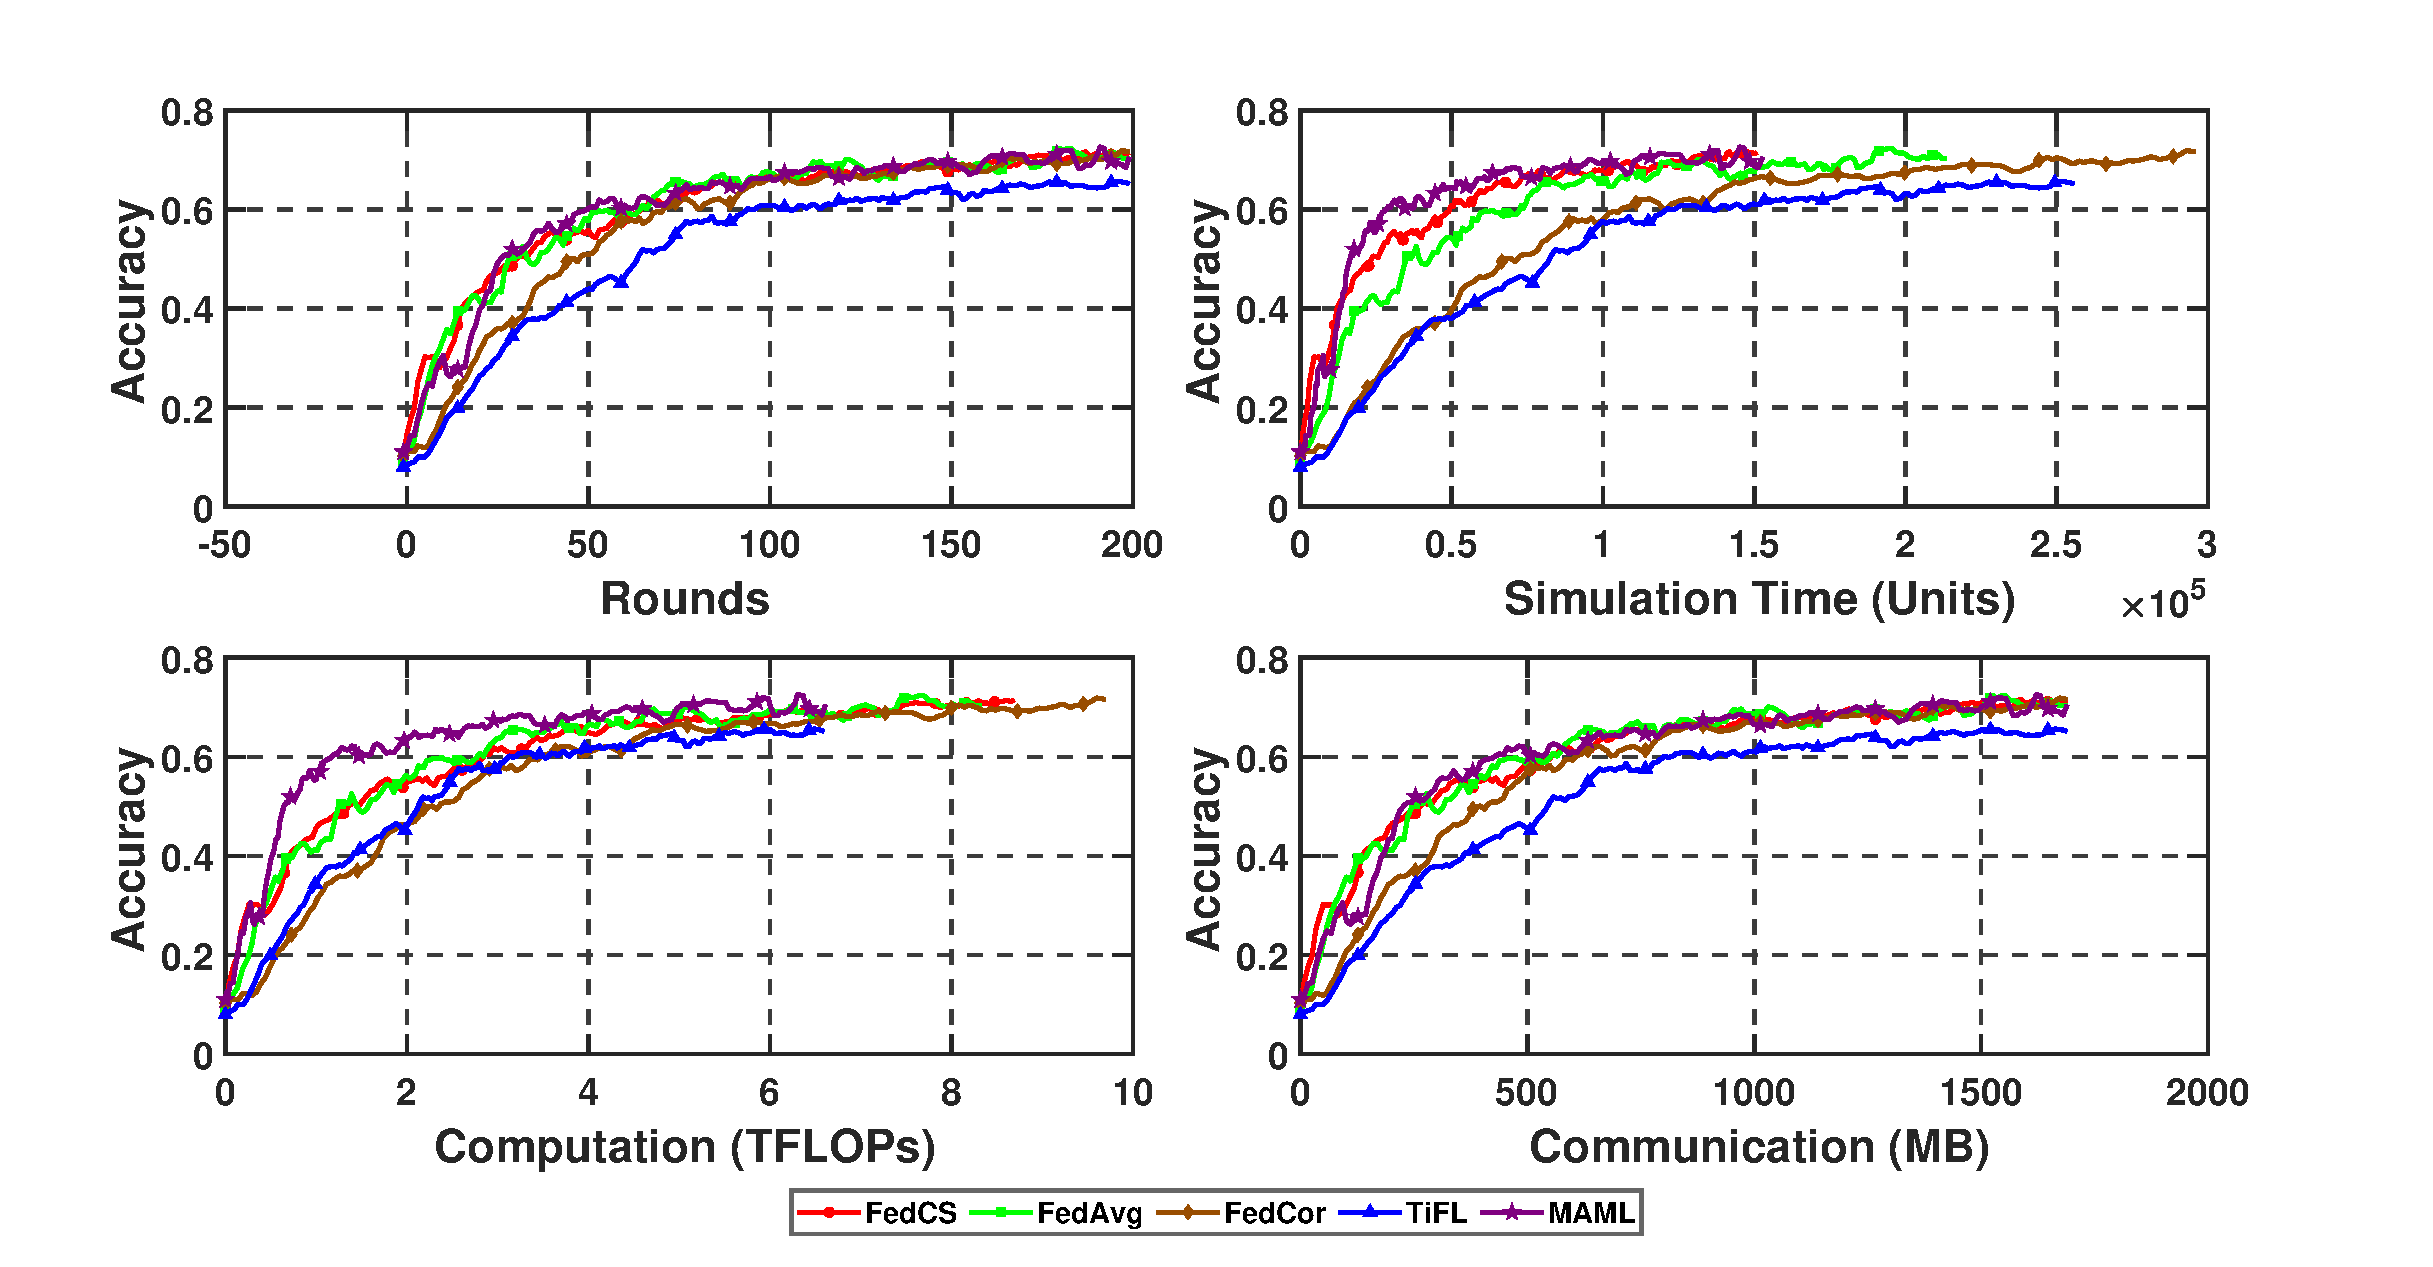
\includegraphics[width=\columnwidth]{Fashion_mnist_efficiency_new.eps}
		\vspace{0.3em}
		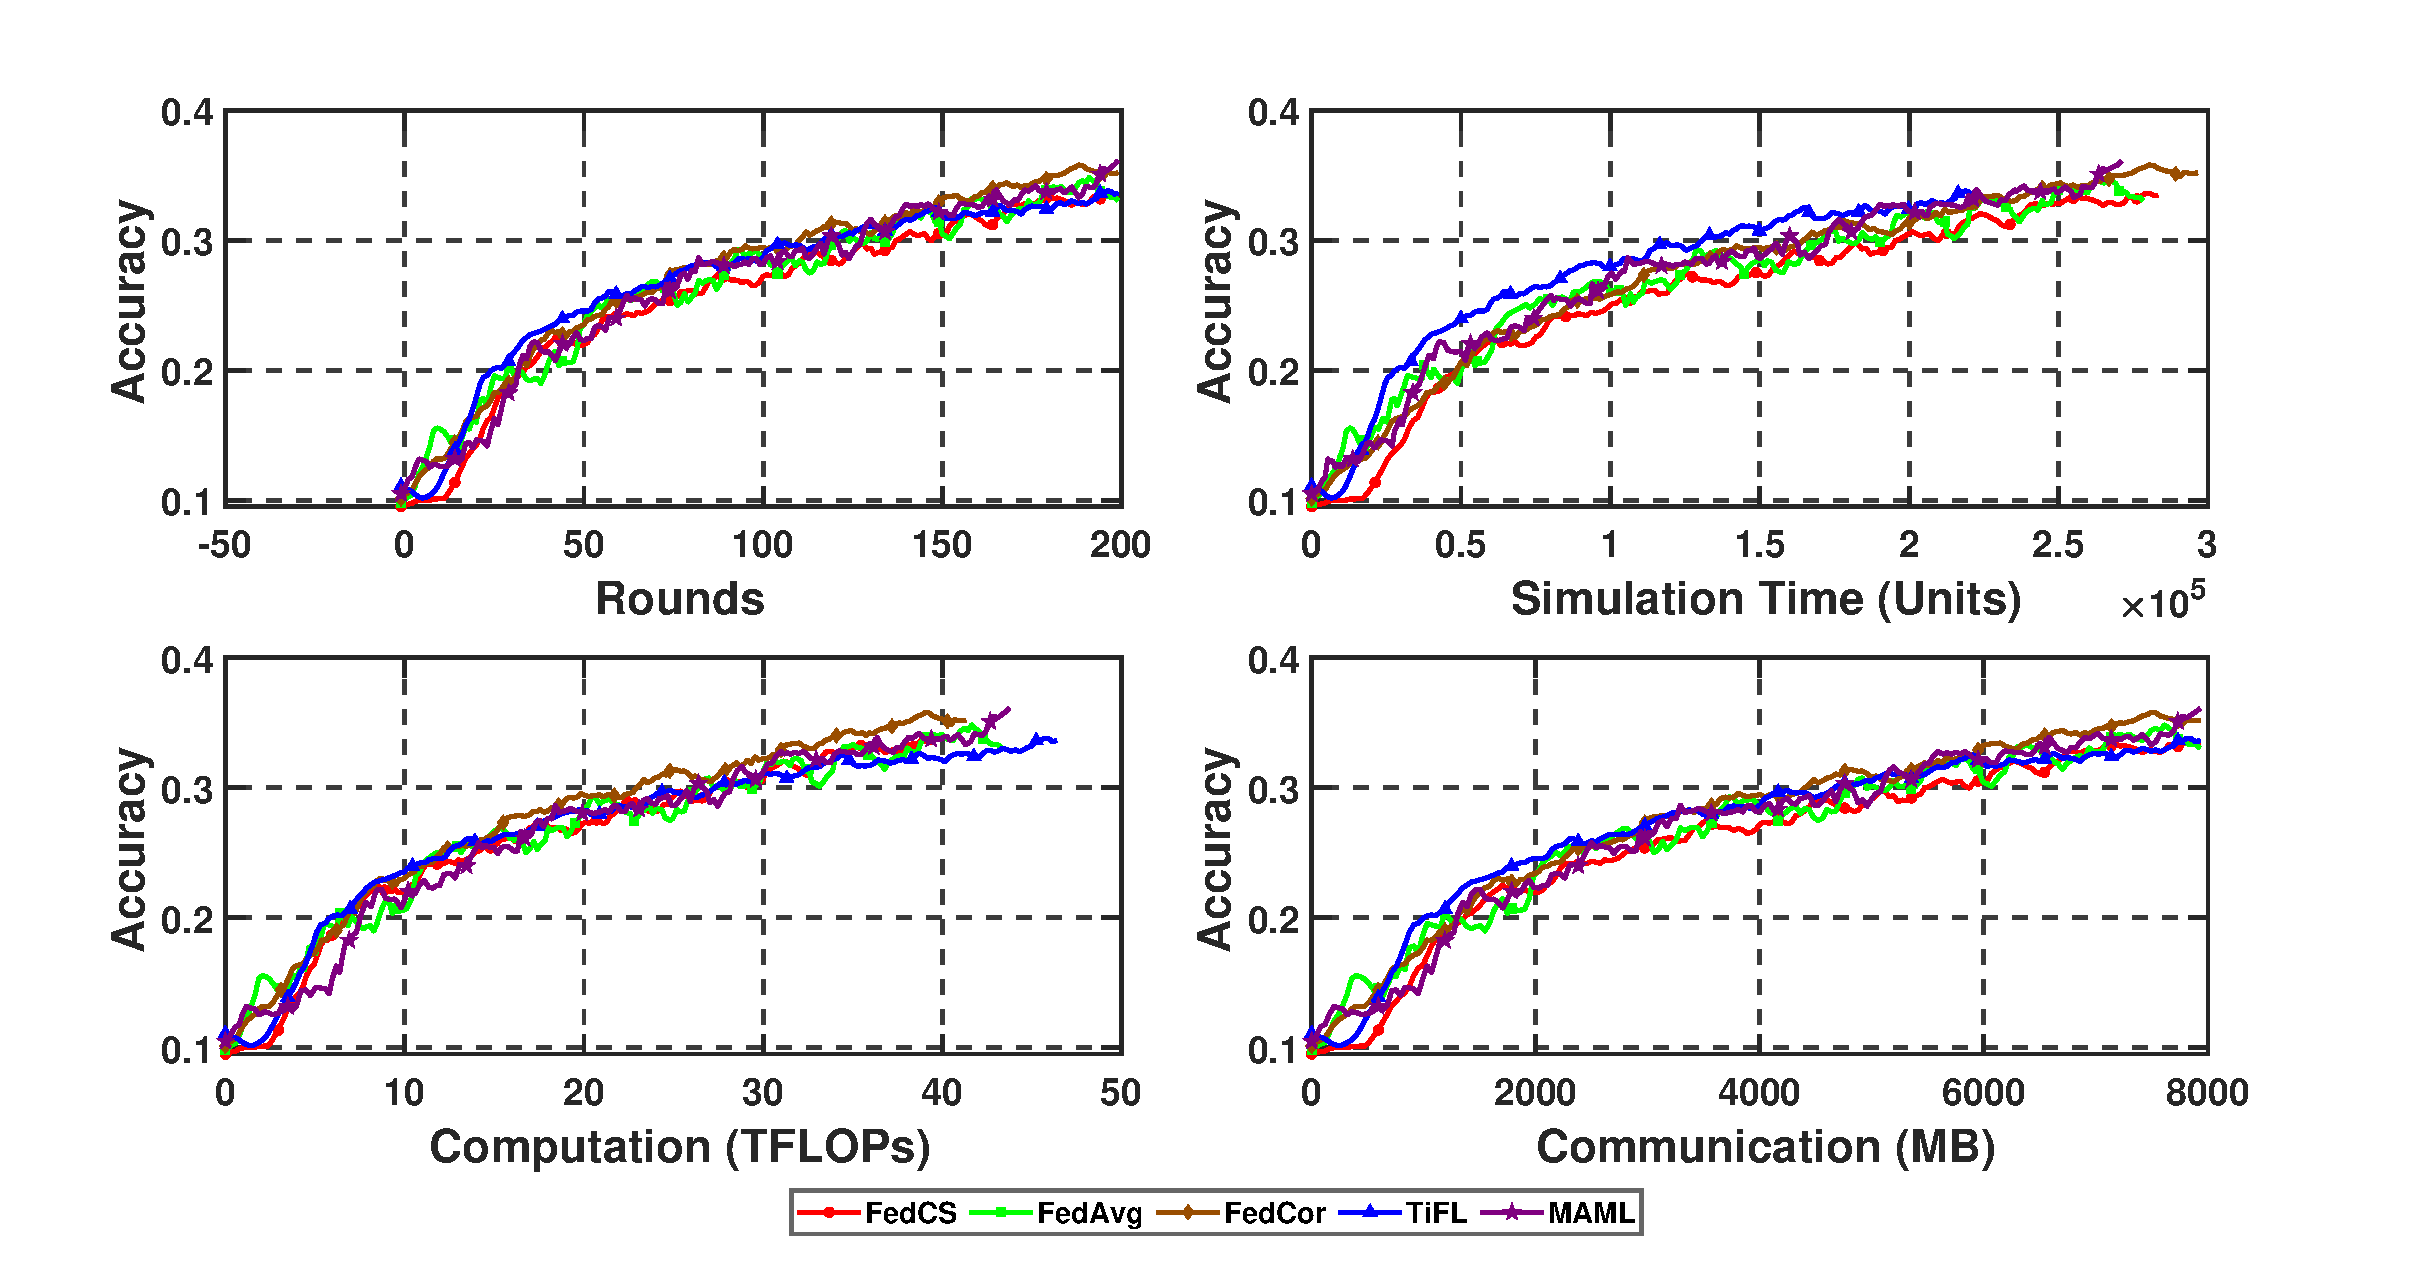
\includegraphics[width=\columnwidth]{cifar_10_efficiency_new.eps}
		\caption{\small \revision{Current efficiency comparison. Top: Fashion-MNIST. Bottom: CIFAR-10. Simulation time is accumulated modeled latency. TFLOPs are cumulative client-training operations.}}
	\label{fig:efficiency_comparison}
\end{figure}

\subsection{Performance Summary}
\revision{Table~\ref{tab:performance_summary} reports the current single-run summary averaged over the last 10 rounds. On CIFAR-10, MAML-Select improves accuracy by 1.39 percentage points over random FedAvg selection. On Fashion-MNIST, it improves accuracy by 0.65 percentage points and reduces simulated time by 28.5\%. These results motivate expanded evaluation with repeated runs, uncertainty reporting, feature ablations, fairness metrics, and direct comparisons with recent selectors.}

\begin{table}[!t]
		\caption{\small \revision{Current performance summary on Fashion-MNIST and CIFAR-10 (averaged over the last 10 rounds).}}
	\centering
	\resizebox{\columnwidth}{!}{
		\begin{tabular}{@{}l|cc|cc@{}}
			\toprule
			\textbf{Dataset} & \multicolumn{2}{c|}{\textbf{Fashion-MNIST}} & \multicolumn{2}{c}{\textbf{CIFAR-10}} \\
			\cmidrule{2-5}
				\textbf{Metric} & \textbf{FedAvg} & \textbf{\revision{MAML-Select}} & \textbf{FedAvg} & \textbf{\revision{MAML-Select}} \\
			\midrule
			Accuracy (\%) & 70.42 & \textbf{71.07} & 33.85 & \textbf{35.24} \\
			F1-Score       & 0.6837 & \textbf{0.6841} & 0.3100 & \textbf{0.3097} \\
			Precision      & 0.6901 & 0.6912 & 0.3205 & \textit{0.3310} \\
			Recall         & 0.6780 & \textbf{0.6815} & 0.3015 & \textbf{0.3150} \\
			\midrule
				\revision{Sim. time (arb. units)}  & 2.14e5 & \textbf{1.53e5} & 2.78e5 & 2.96e5 \\
			Comp. (TFLOPs) & 8.33  & \textbf{6.61} & 43.32 & 41.32 \\
			\bottomrule
				\multicolumn{5}{l}{\footnotesize \revision{Bold values indicate the better value within each dataset pair.}}
		\end{tabular}
	}
	\label{tab:performance_summary}
\end{table}

% =====================================================================
% VI. CONCLUSION
% =====================================================================
\section{Conclusion and Future Work}
\revision{We introduced MAML-Select, an online adaptive client-selection framework for heterogeneous FL. The method learns an initialization for a lightweight ranking policy and adapts it from recent feedback before each selection decision. Current experiments on Fashion-MNIST and CIFAR-10 indicate lower cumulative computation, faster convergence, and modest accuracy gains over random FedAvg selection. These metrics are computational proxies rather than direct measurements of energy use. Future work will extend the evaluation to larger benchmarks, repeated runs, fairness analysis, feature ablations, and hardware-level measurements.}

% =====================================================================
% REFERENCES
% =====================================================================
\balance
\FloatBarrier
\bibliographystyle{IEEEtran}
\bibliography{References_letter}

\end{document}
